\chapter{Eindimensionale Potentialprobleme}

\section{Ziel dieses Kapitels}

In diesem Kapitel geht es darum, wie man die zeitunabhängige Schrödingergleichung in einer Raumdimension für einfache Potentiale löst. Diese Aufgaben sind in der Quantenmechanik besonders wichtig, weil sie die Grundideen von gebundenen Zuständen, Streuzuständen, Reflexion, Transmission und Tunneleffekt in einer mathematisch kontrollierbaren Form zeigen.

Die zentralen Fragen sind:
\begin{itemize}
    \item Wie reduziert man die zeitabhängige Schrödingergleichung auf ein Energieeigenwertproblem?
    \item Welche Rand- und Anschlussbedingungen müssen Wellenfunktionen erfüllen?
    \item Was ist der Unterschied zwischen gebundenen Zuständen und Streuzuständen?
    \item Wie berechnet man Reflexions- und Transmissionswahrscheinlichkeiten?
    \item Warum kann ein Teilchen an einer Potentialstufe reflektiert werden, obwohl es klassisch genügend Energie besitzt?
    \item Warum kann ein Teilchen eine Potentialbarriere durchdringen, obwohl seine Energie kleiner als die Barrierenhöhe ist?
    \item Wie entstehen diskrete Energien im Potentialtopf?
    \item Wie behandelt man Delta-Potentiale und warum springt dort die Ableitung der Wellenfunktion?
\end{itemize}

\begin{conceptbox}
Eindimensionale Potentialprobleme sind der erste Ort, an dem der Unterschied zwischen klassischer Mechanik und Quantenmechanik wirklich sichtbar wird. Klassisch bewegt sich ein Teilchen entweder über eine Barriere oder nicht. Quantenmechanisch wird eine Welle an jedem Potentialwechsel teilweise reflektiert, teilweise transmittiert oder exponentiell gedämpft. Dadurch entstehen Effekte wie partielle Reflexion, Tunneleffekt und diskrete gebundene Zustände.
\end{conceptbox}

\section{Allgemeine Problemstellung}

\subsection{Zeitabhängige Schrödingergleichung in einer Dimension}

Wir betrachten ein Teilchen der Masse $m$ in einer Raumdimension mit Potential $V(x)$. Der Hamiltonoperator lautet
\[
    H=-\frac{\hbar^2}{2m}\frac{\dd^2}{\dd x^2}+V(x).
\]
Die zeitabhängige Schrödingergleichung ist
\[
    i\hbar\frac{\partial}{\partial t}\psi(x,t)
    =H\psi(x,t)
    =\left(-\frac{\hbar^2}{2m}\frac{\partial^2}{\partial x^2}+V(x)\right)\psi(x,t).
\]
Wenn das Potential nicht explizit von der Zeit abhängt, kann man stationäre Zustände suchen.

\begin{definitionbox}
Ein Potentialproblem heißt zeitunabhängig, wenn
\[
    V=V(x)
\]
gilt und keine explizite Zeitabhängigkeit vorhanden ist. Dann ist auch der Hamiltonoperator zeitunabhängig.
\end{definitionbox}

\subsection{Separationsansatz}

Für zeitunabhängige Hamiltonoperatoren verwendet man den Separationsansatz
\[
    \psi(x,t)=\varphi(x)\mathrm{e}^{-iEt/\hbar}.
\]
Dabei ist $E$ eine Energie und $\varphi(x)$ die zeitunabhängige Ortswellenfunktion.

\begin{derivationbox}
Wir setzen
\[
    \psi(x,t)=\varphi(x)\mathrm{e}^{-iEt/\hbar}
\]
in die zeitabhängige Schrödingergleichung ein. Die linke Seite ist
\[
    i\hbar\frac{\partial}{\partial t}\psi(x,t)
    =i\hbar\left(-\frac{iE}{\hbar}\right)\varphi(x)\mathrm{e}^{-iEt/\hbar}
    =E\varphi(x)\mathrm{e}^{-iEt/\hbar}.
\]
Die rechte Seite ist
\[
    H\psi(x,t)=\left(H\varphi(x)\right)\mathrm{e}^{-iEt/\hbar}.
\]
Da der Exponentialfaktor nie verschwindet, folgt
\[
    H\varphi(x)=E\varphi(x).
\]
Damit wird aus der zeitabhängigen Schrödingergleichung das zeitunabhängige Eigenwertproblem.
\end{derivationbox}

\begin{formulabox}
Die zeitunabhängige Schrödingergleichung in einer Dimension lautet
\[
    -\frac{\hbar^2}{2m}\varphi''(x)+V(x)\varphi(x)=E\varphi(x).
\]
Äquivalent:
\[
    \varphi''(x)+\frac{2m}{\hbar^2}\bigl(E-V(x)\bigr)\varphi(x)=0.
\]
\end{formulabox}

\subsection{Physikalische Bedeutung der Energieeigenfunktionen}

Wenn
\[
    H\varphi_n=E_n\varphi_n
\]
gilt, dann ist
\[
    \psi_n(x,t)=\varphi_n(x)\mathrm{e}^{-iE_nt/\hbar}
\]
ein stationärer Zustand. Die Aufenthaltswahrscheinlichkeit ist zeitunabhängig:
\[
    |\psi_n(x,t)|^2
    =|\varphi_n(x)|^2\left|\mathrm{e}^{-iE_nt/\hbar}\right|^2
    =|\varphi_n(x)|^2.
\]

\begin{notebox}
Stationär bedeutet nicht, dass die Wellenfunktion selbst zeitunabhängig ist. Die Wellenfunktion besitzt einen zeitabhängigen Phasenfaktor. Aber alle Wahrscheinlichkeitsdichten und Erwartungswerte zeitunabhängiger Observablen, die mit $H$ kompatibel sind, bleiben in einem Energieeigenzustand konstant.
\end{notebox}

\section{Gebundene Zustände und Streuzustände}

\subsection{Gebundene Zustände}

Ein gebundener Zustand ist ein Zustand, dessen Wellenfunktion räumlich lokalisiert und quadratintegrierbar ist:
\[
    \int_{-\infty}^{\infty}\dd x\,|\varphi(x)|^2<\infty.
\]
Nach Normierung gilt
\[
    \int_{-\infty}^{\infty}\dd x\,|\varphi(x)|^2=1.
\]

\begin{definitionbox}
Ein gebundener Zustand ist ein normalisierbarer Energieeigenzustand. Er gehört typischerweise zu einem diskreten Energiespektrum.
\end{definitionbox}

Physikalisch bedeutet das: Das Teilchen bleibt mit Wahrscheinlichkeit $1$ in einem endlichen Bereich lokalisiert, wenn man weit genug nach außen geht.

Typische Beispiele:
\begin{itemize}
    \item Teilchen im unendlich hohen Kasten,
    \item gebundene Zustände im endlichen Potentialtopf,
    \item gebundener Zustand im attraktiven Delta-Potential,
    \item Elektron in einem gebundenen atomaren Zustand.
\end{itemize}

\subsection{Streuzustände}

Ein Streuzustand beschreibt ein Teilchen, das aus dem Unendlichen kommt und nach Wechselwirkung mit dem Potential wieder ins Unendliche läuft. Solche Zustände sind in der Regel nicht quadratintegrierbar, sondern delta-normalisiert oder als Wellenpakete zu verstehen.

\begin{definitionbox}
Ein Streuzustand ist ein Energieeigenzustand des kontinuierlichen Spektrums. Er ist meistens nicht in $L^2(\R)$ normalisierbar und wird physikalisch als Idealisierung eines Wellenpakets verstanden.
\end{definitionbox}

Typische Beispiele:
\begin{itemize}
    \item Streuung an einer Potentialstufe,
    \item Streuung an einer Potentialbarriere,
    \item Streuung an einem Potentialtopf,
    \item Streuung an einem Delta-Potential.
\end{itemize}

\begin{conceptbox}
Der Unterschied zwischen gebundenen Zuständen und Streuzuständen ist nicht nur mathematisch. Gebundene Zustände haben diskrete Energien und sind lokalisierbar. Streuzustände haben kontinuierliche Energien und beschreiben einlaufende, reflektierte und transmittierte Wellen.
\end{conceptbox}

\section{Lösung in Bereichen konstanten Potentials}

Viele Standardprobleme haben ein stückweise konstantes Potential. In jedem Bereich ist $V(x)$ konstant. Dann kann man die Schrödingergleichung explizit lösen und anschließend die Lösungen an den Grenzstellen zusammenkleben.

Sei in einem Bereich
\[
    V(x)=V_c=\text{konstant}.
\]
Dann lautet die zeitunabhängige Schrödingergleichung
\[
    -\frac{\hbar^2}{2m}\varphi''(x)+V_c\varphi(x)=E\varphi(x).
\]
Also
\[
    \varphi''(x)+\frac{2m}{\hbar^2}(E-V_c)\varphi(x)=0.
\]

\subsection{Fall $E>V_c$: oszillatorische Lösung}

Ist
\[
    E>V_c,
\]
dann definiert man
\[
    k=\frac{\sqrt{2m(E-V_c)}}{\hbar}.
\]
Die Gleichung wird
\[
    \varphi''(x)+k^2\varphi(x)=0.
\]
Die allgemeine Lösung ist
\[
    \varphi(x)=A\mathrm{e}^{ikx}+B\mathrm{e}^{-ikx}.
\]

\begin{notebox}
Der Term $\mathrm{e}^{ikx}$ beschreibt eine nach rechts laufende Welle, wenn der Zeitfaktor $\mathrm{e}^{-iEt/\hbar}$ mitgenommen wird. Der Term $\mathrm{e}^{-ikx}$ beschreibt eine nach links laufende Welle.
\end{notebox}

\subsection{Fall $E<V_c$: exponentielle Lösung}

Ist
\[
    E<V_c,
\]
dann definiert man
\[
    \kappa=\frac{\sqrt{2m(V_c-E)}}{\hbar}.
\]
Die Gleichung wird
\[
    \varphi''(x)-\kappa^2\varphi(x)=0.
\]
Die allgemeine Lösung ist
\[
    \varphi(x)=C\mathrm{e}^{\kappa x}+D\mathrm{e}^{-\kappa x}.
\]

\begin{conceptbox}
In klassisch verbotenen Bereichen, also dort wo $E<V(x)$ gilt, wird die Wellenfunktion nicht sofort null. Sie fällt exponentiell ab oder wächst exponentiell an. Für physikalische gebundene Zustände muss man die wachsenden Terme im Unendlichen verwerfen. Für Barrieren endlicher Breite ist der exponentielle Anteil aber entscheidend: Er ermöglicht den Tunneleffekt.
\end{conceptbox}

\subsection{Fall $E=V_c$}

Ist
\[
    E=V_c,
\]
dann gilt
\[
    \varphi''(x)=0.
\]
Die allgemeine Lösung ist linear:
\[
    \varphi(x)=A+Bx.
\]
Dieser Spezialfall tritt als Grenzfall zwischen oszillatorischem und exponentiellem Verhalten auf.

\section{Anschlussbedingungen}

\subsection{Endliche Potentialsprünge}

Bei stückweise konstanten Potentialen treten Sprungstellen auf. Sei $x=a$ eine Stelle, an der das Potential zwar springt, aber endlich bleibt. Dann gelten die Anschlussbedingungen
\[
    \varphi(a^-)=\varphi(a^+),
    \qquad
    \varphi'(a^-)=\varphi'(a^+).
\]

\begin{derivationbox}
Die Stetigkeit der Ableitung folgt aus der integrierten Schrödingergleichung. Wir integrieren über ein kleines Intervall $[a-\varepsilon,a+\varepsilon]$:
\[
    \int_{a-\varepsilon}^{a+\varepsilon}\dd x
    \left(-\frac{\hbar^2}{2m}\varphi''(x)+V(x)\varphi(x)\right)
    =\int_{a-\varepsilon}^{a+\varepsilon}\dd x\,E\varphi(x).
\]
Der kinetische Term ergibt
\[
    -\frac{\hbar^2}{2m}\left[\varphi'(a+\varepsilon)-\varphi'(a-\varepsilon)\right].
\]
Wenn $V(x)$ endlich ist und $\varphi(x)$ beschränkt bleibt, verschwinden die Potential- und Energieterme im Limes $\varepsilon\to0$. Damit folgt
\[
    \varphi'(a^+)-\varphi'(a^-)=0.
\]
Also ist $\varphi'$ stetig.
\end{derivationbox}

\begin{formulabox}
Für endliche Potentialsprünge gilt:
\[
    \boxed{\varphi(a^-)=\varphi(a^+)},
    \qquad
    \boxed{\varphi'(a^-)=\varphi'(a^+)}.
\]
\end{formulabox}

\subsection{Unendlich hohe Wände}

Bei einer unendlich hohen Wand kann das Teilchen den verbotenen Bereich nicht betreten. Ist zum Beispiel
\[
    V(x)=\infty
\]
außerhalb eines Intervalls, dann muss die Wellenfunktion dort verschwinden. An der Wand gilt daher
\[
    \varphi=0.
\]

\begin{notebox}
Bei einer unendlich hohen Wand ist die Ableitung der Wellenfunktion im Allgemeinen nicht stetig. Die Wand ist kein endlicher Potentialsprung, sondern ein Grenzfall eines unendlich großen Potentials.
\end{notebox}

\subsection{Delta-Potentiale}

Ein Delta-Potential hat die Form
\[
    V(x)=\lambda\delta(x-a).
\]
Hier ist das Potential an einer Stelle singulär. Die Wellenfunktion bleibt stetig, aber ihre Ableitung springt.

\begin{derivationbox}
Wir betrachten
\[
    H=-\frac{\hbar^2}{2m}\frac{\dd^2}{\dd x^2}+\lambda\delta(x-a).
\]
Die Eigenwertgleichung ist
\[
    -\frac{\hbar^2}{2m}\varphi''(x)+\lambda\delta(x-a)\varphi(x)=E\varphi(x).
\]
Integration von $a-\varepsilon$ bis $a+\varepsilon$ liefert
\[
    -\frac{\hbar^2}{2m}\left[\varphi'(a^+)-\varphi'(a^-)\right]
    +\lambda\varphi(a)
    =E\int_{a-\varepsilon}^{a+\varepsilon}\dd x\,\varphi(x).
\]
Im Limes $\varepsilon\to0$ verschwindet die rechte Seite. Also
\[
    -\frac{\hbar^2}{2m}\left[\varphi'(a^+)-\varphi'(a^-)\right]
    +\lambda\varphi(a)=0.
\]
Damit folgt
\[
    \varphi'(a^+)-\varphi'(a^-)
    =\frac{2m\lambda}{\hbar^2}\varphi(a).
\]
\end{derivationbox}

\begin{formulabox}
Für ein Delta-Potential $V(x)=\lambda\delta(x-a)$ gilt
\[
    \boxed{\varphi(a^-)=\varphi(a^+)},
\]
aber
\[
    \boxed{\varphi'(a^+)-\varphi'(a^-)=\frac{2m\lambda}{\hbar^2}\varphi(a)}.
\]
Für ein attraktives Delta-Potential $V(x)=-\alpha\delta(x)$ mit $\alpha>0$ ist also
\[
    \varphi'(0^+)-\varphi'(0^-)
    =-\frac{2m\alpha}{\hbar^2}\varphi(0).
\]
\end{formulabox}

\section{Wahrscheinlichkeitsstrom, Reflexion und Transmission}

\subsection{Wahrscheinlichkeitsstrom in einer Dimension}

Für eine Wellenfunktion $\psi(x,t)$ ist der Wahrscheinlichkeitsstrom
\[
    j(x,t)=\frac{\hbar}{2mi}\left(\psi^*\frac{\partial\psi}{\partial x}-\psi\frac{\partial\psi^*}{\partial x}\right).
\]
Äquivalent:
\[
    j(x,t)=\frac{\hbar}{m}\operatorname{Im}\left(\psi^*\frac{\partial\psi}{\partial x}\right).
\]

Für eine stationäre ebene Welle
\[
    \psi(x,t)=A\mathrm{e}^{ikx}\mathrm{e}^{-iEt/\hbar}
\]
gilt
\begin{derivationbox}
\[
    \frac{\partial\psi}{\partial x}=ik\psi.
\]
Damit
\[
    j=\frac{\hbar}{m}\operatorname{Im}(\psi^*ik\psi)
    =\frac{\hbar}{m}\operatorname{Im}(ik|\psi|^2)
    =\frac{\hbar k}{m}|A|^2.
\]
\end{derivationbox}

Für eine nach links laufende Welle $A\mathrm{e}^{-ikx}$ erhält man entsprechend
\[
    j=-\frac{\hbar k}{m}|A|^2.
\]

\begin{formulabox}
Eine ebene Welle $A\mathrm{e}^{ikx}$ trägt den Strom
\[
    j=\frac{\hbar k}{m}|A|^2.
\]
Eine ebene Welle $A\mathrm{e}^{-ikx}$ trägt den Strom
\[
    j=-\frac{\hbar k}{m}|A|^2.
\]
\end{formulabox}

\subsection{Reflexions- und Transmissionskoeffizient}

Bei einem Streuproblem von links schreibt man asymptotisch häufig
\[
    \varphi(x)=
    \begin{cases}
        A\mathrm{e}^{ik_1x}+B\mathrm{e}^{-ik_1x}, & x\to -\infty,\\
        F\mathrm{e}^{ik_2x}, & x\to +\infty.
    \end{cases}
\]
Dabei ist $A$ die einlaufende Amplitude, $B$ die reflektierte Amplitude und $F$ die transmittierte Amplitude.

Der Reflexionskoeffizient ist
\[
    R=\frac{|j_{\mathrm{ref}}|}{|j_{\mathrm{ein}}|}.
\]
Der Transmissionskoeffizient ist
\[
    T=\frac{|j_{\mathrm{trans}}|}{|j_{\mathrm{ein}}|}.
\]

Da die Stromdichte proportional zu $k|A|^2$ ist, gilt
\[
    R=\left|\frac{B}{A}\right|^2,
\]
aber
\[
    T=\frac{k_2}{k_1}\left|\frac{F}{A}\right|^2.
\]

\begin{notebox}
Man darf $T$ nicht immer einfach mit $|F/A|^2$ identifizieren. Wenn links und rechts verschiedene Wellenzahlen auftreten, muss der Geschwindigkeitsfaktor $k_2/k_1$ mitgenommen werden. Nur wenn $k_1=k_2$ gilt, ist $T=|F/A|^2$.
\end{notebox}

\begin{formulabox}
Für Streuung von links mit Wellenzahlen $k_1$ links und $k_2$ rechts gilt
\[
    R=\left|\frac{B}{A}\right|^2,
    \qquad
    T=\frac{k_2}{k_1}\left|\frac{F}{A}\right|^2.
\]
Für ein reelles zeitunabhängiges Potential gilt bei eindimensionaler Streuung
\[
    R+T=1.
\]
\end{formulabox}

\section{Potentialstufe}

\subsection{Definition des Potentials}

Die Potentialstufe ist definiert durch
\[
    V(x)=
    \begin{cases}
        0, & x<0,\\
        V_0, & x>0,
    \end{cases}
    \qquad V_0>0.
\]
Wir betrachten ein Teilchen, das von links auf die Stufe trifft.

\begin{center}
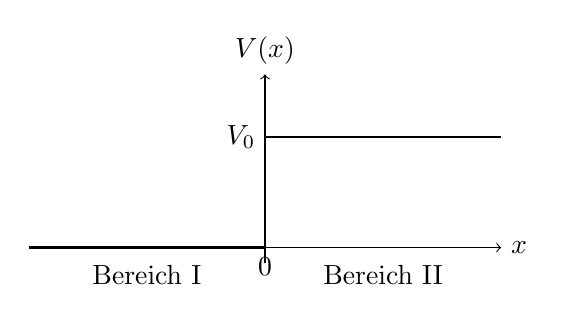
\begin{tikzpicture}[scale=1.0]
    \draw[->] (-3,0) -- (3,0) node[right] {$x$};
    \draw[->] (0,-0.2) -- (0,2.2) node[above] {$V(x)$};
    \draw[thick] (-3,0) -- (0,0) -- (0,1.4) -- (3,1.4);
    \node[left] at (0,1.4) {$V_0$};
    \node[below] at (0,0) {$0$};
    \node at (-1.5,-0.35) {Bereich I};
    \node at (1.5,-0.35) {Bereich II};
\end{tikzpicture}
\end{center}

\subsection{Fall $E>V_0$: partielle Reflexion und Transmission}

Für $E>V_0$ ist die Bewegung in beiden Bereichen klassisch erlaubt. Wir definieren
\[
    k_1=\frac{\sqrt{2mE}}{\hbar},
    \qquad
    k_2=\frac{\sqrt{2m(E-V_0)}}{\hbar}.
\]
Ein von links einlaufender Zustand hat die Form
\[
    \varphi_I(x)=\mathrm{e}^{ik_1x}+r\mathrm{e}^{-ik_1x},
    \qquad x<0,
\]
\[
    \varphi_{II}(x)=t\mathrm{e}^{ik_2x},
    \qquad x>0.
\]
Dabei wurde die einlaufende Amplitude auf $1$ gesetzt. Die Koeffizienten $r$ und $t$ heißen Reflexions- und Transmissionsamplitude.

\begin{derivationbox}
An $x=0$ gelten Stetigkeit von $\varphi$ und $\varphi'$:
\[
    \varphi_I(0)=\varphi_{II}(0),
    \qquad
    \varphi_I'(0)=\varphi_{II}'(0).
\]
Aus der Wellenfunktion folgt
\[
    1+r=t.
\]
Aus der Ableitung folgt
\[
    ik_1(1-r)=ik_2t.
\]
Also
\[
    k_1(1-r)=k_2(1+r).
\]
Damit
\[
    k_1-k_1r=k_2+k_2r,
\]
und daher
\[
    r=\frac{k_1-k_2}{k_1+k_2}.
\]
Weiter ist
\[
    t=1+r=1+\frac{k_1-k_2}{k_1+k_2}
    =\frac{2k_1}{k_1+k_2}.
\]
\end{derivationbox}

\begin{formulabox}
Für die Potentialstufe mit $E>V_0$ und Einfall von links gilt
\[
    r=\frac{k_1-k_2}{k_1+k_2},
    \qquad
    t=\frac{2k_1}{k_1+k_2}.
\]
Die Wahrscheinlichkeiten sind
\[
    R=|r|^2=\left(\frac{k_1-k_2}{k_1+k_2}\right)^2,
\]
\[
    T=\frac{k_2}{k_1}|t|^2
    =\frac{4k_1k_2}{(k_1+k_2)^2}.
\]
Es gilt
\[
    R+T=1.
\]
\end{formulabox}

\begin{conceptbox}
Klassisch würde ein Teilchen mit $E>V_0$ einfach über die Stufe laufen. Quantenmechanisch wird es teilweise reflektiert. Diese Reflexion entsteht nicht, weil das Teilchen zu wenig Energie hat, sondern weil die Wellenzahl an der Stufe springt und die Wellenfunktion samt Ableitung angepasst werden muss.
\end{conceptbox}

\subsection{Fall $0<E<V_0$: totale Reflexion mit Eindringen}

Für $0<E<V_0$ ist der Bereich $x>0$ klassisch verboten. Wir definieren
\[
    k=\frac{\sqrt{2mE}}{\hbar},
    \qquad
    \kappa=\frac{\sqrt{2m(V_0-E)}}{\hbar}.
\]
Der Ansatz lautet
\[
    \varphi_I(x)=\mathrm{e}^{ikx}+r\mathrm{e}^{-ikx},
    \qquad x<0,
\]
\[
    \varphi_{II}(x)=C\mathrm{e}^{-\kappa x},
    \qquad x>0.
\]
Der wachsende Term $\mathrm{e}^{+\kappa x}$ wird verworfen, weil er für $x\to+\infty$ divergiert.

\begin{derivationbox}
Die Anschlussbedingungen bei $x=0$ liefern
\[
    1+r=C,
\]
und
\[
    ik(1-r)=-\kappa C.
\]
Einsetzen von $C=1+r$ ergibt
\[
    ik(1-r)=-\kappa(1+r).
\]
Also
\[
    ik-ikr=-\kappa-\kappa r.
\]
Damit
\[
    r(\kappa-ik)=-(\kappa+ik).
\]
Also
\[
    r=\frac{ik+\kappa}{ik-\kappa}
    =\frac{k-i\kappa}{k+i\kappa}.
\]
Daraus folgt
\[
    |r|^2=1.
\]
\end{derivationbox}

\begin{formulabox}
Für die Potentialstufe mit $0<E<V_0$ gilt
\[
    R=1,
    \qquad
    T=0.
\]
Die Wellenfunktion dringt aber in den klassisch verbotenen Bereich ein:
\[
    \varphi_{II}(x)=C\mathrm{e}^{-\kappa x}.
\]
Die Eindringtiefe ist von der Größenordnung
\[
    \ell\sim\frac{1}{\kappa}
    =\frac{\hbar}{\sqrt{2m(V_0-E)}}.
\]
\end{formulabox}

\begin{conceptbox}
Bei $0<E<V_0$ gibt es totale Reflexion, aber die Wellenfunktion ist im verbotenen Bereich nicht null. Das ist ein rein quantenmechanischer Effekt. Bei einer unendlich breiten Stufe kommt kein Strom nach rechts, aber die Wahrscheinlichkeitsamplitude dringt exponentiell in die Stufe ein.
\end{conceptbox}

\section{Potentialbarriere und Tunneleffekt}

\subsection{Definition der Barriere}

Eine rechteckige Potentialbarriere ist definiert durch
\[
    V(x)=
    \begin{cases}
        0, & x<0,\\
        V_0, & 0\le x\le L,\\
        0, & x>L,
    \end{cases}
    \qquad V_0>0.
\]
In manchen Aufgaben wird die Breite als $2a$ geschrieben. Dann gilt einfach $L=2a$.

\begin{center}
\begin{tikzpicture}[scale=1.0]
    \draw[->] (-3,0) -- (4,0) node[right] {$x$};
    \draw[->] (0,-0.2) -- (0,2.2) node[above] {$V(x)$};
    \draw[thick] (-3,0) -- (0,0) -- (0,1.4) -- (2,1.4) -- (2,0) -- (4,0);
    \node[left] at (0,1.4) {$V_0$};
    \node[below] at (0,0) {$0$};
    \node[below] at (2,0) {$L$};
    \node at (-1.5,-0.35) {I};
    \node at (1,-0.35) {II};
    \node at (3,-0.35) {III};
\end{tikzpicture}
\end{center}

Wir betrachten Einfall von links. Für $x<0$ gibt es eine einlaufende und eine reflektierte Welle. Für $x>L$ gibt es nur eine nach rechts laufende transmittierte Welle.

\subsection{Fall $0<E<V_0$: Tunneln}

Für $0<E<V_0$ definieren wir
\[
    k=\frac{\sqrt{2mE}}{\hbar},
    \qquad
    \kappa=\frac{\sqrt{2m(V_0-E)}}{\hbar}.
\]
Der Ansatz lautet
\[
    \varphi_I(x)=A\mathrm{e}^{ikx}+B\mathrm{e}^{-ikx},
    \qquad x<0,
\]
\[
    \varphi_{II}(x)=C\mathrm{e}^{\kappa x}+D\mathrm{e}^{-\kappa x},
    \qquad 0\le x\le L,
\]
\[
    \varphi_{III}(x)=F\mathrm{e}^{ikx},
    \qquad x>L.
\]

\begin{notebox}
Im Barrierenbereich braucht man im Allgemeinen beide Exponentialterme. Obwohl $\mathrm{e}^{\kappa x}$ wächst, ist der Bereich endlich. Der Term ist deshalb nicht automatisch verboten. Erst in einem unendlichen verbotenen Bereich müsste man den wachsenden Term verwerfen.
\end{notebox}

Die vier Anschlussbedingungen sind
\[
    \varphi_I(0)=\varphi_{II}(0),
    \qquad
    \varphi_I'(0)=\varphi_{II}'(0),
\]
\[
    \varphi_{II}(L)=\varphi_{III}(L),
    \qquad
    \varphi_{II}'(L)=\varphi_{III}'(L).
\]
Daraus ergibt sich nach algebraischer Rechnung der Transmissionskoeffizient.

\begin{formulabox}
Für eine rechteckige Barriere der Breite $L$ mit $0<E<V_0$ gilt
\[
    T(E)=\left[1+\frac{V_0^2}{4E(V_0-E)}\sinh^2(\kappa L)\right]^{-1},
\]
mit
\[
    \kappa=\frac{\sqrt{2m(V_0-E)}}{\hbar}.
\]
\end{formulabox}

\begin{conceptbox}
Klassisch wäre für $E<V_0$ die Transmission durch die Barriere unmöglich. Quantenmechanisch ist sie möglich, weil die Wellenfunktion im Inneren der Barriere nur exponentiell gedämpft wird und bei endlicher Breite auf der anderen Seite noch eine endliche Amplitude übrig bleiben kann. Dieser Effekt heißt Tunneleffekt.
\end{conceptbox}

\subsection{Hohe und breite Barriere}

Für eine hohe und breite Barriere gilt
\[
    \kappa L\gg 1.
\]
Dann ist
\[
    \sinh(\kappa L)\approx \frac{1}{2}\mathrm{e}^{\kappa L},
\]
und daher
\[
    \sinh^2(\kappa L)\approx\frac{1}{4}\mathrm{e}^{2\kappa L}.
\]
Der Transmissionskoeffizient wird näherungsweise
\[
    T(E)\approx
    \frac{16E(V_0-E)}{V_0^2}\mathrm{e}^{-2\kappa L}.
\]

Wenn die Barriere wie im Übungsblatt von $0$ bis $2a$ geht, dann ist $L=2a$ und
\[
    T(E)\approx
    \frac{16E(V_0-E)}{V_0^2}\mathrm{e}^{-4\kappa a}.
\]
Schreibt man
\[
    k=\frac{\sqrt{2mE}}{\hbar},
    \qquad
    \kappa=\frac{\sqrt{2m(V_0-E)}}{\hbar},
\]
dann ist
\[
    \frac{16E(V_0-E)}{V_0^2}
    =\frac{16k^2\kappa^2}{(k^2+\kappa^2)^2}.
\]
Also
\[
    T(E)\approx
    \frac{16k^2\kappa^2}{(k^2+\kappa^2)^2}\mathrm{e}^{-4\kappa a}.
\]

\begin{formulabox}
Für eine sehr hohe und breite Barriere gilt die wichtige Näherung
\[
    T(E)\propto \mathrm{e}^{-2\kappa L},
    \qquad
    \kappa=\frac{\sqrt{2m(V_0-E)}}{\hbar}.
\]
Die Transmission nimmt also exponentiell mit der Barrierenbreite und mit der Wurzel aus der Energiedifferenz $V_0-E$ ab.
\end{formulabox}

\subsection{Fall $E>V_0$: Streuung über der Barriere}

Für $E>V_0$ ist auch der Barrierenbereich klassisch erlaubt. Man definiert
\[
    k=\frac{\sqrt{2mE}}{\hbar},
    \qquad
    q=\frac{\sqrt{2m(E-V_0)}}{\hbar}.
\]
Dann ist der Ansatz
\[
    \varphi_I(x)=A\mathrm{e}^{ikx}+B\mathrm{e}^{-ikx},
\]
\[
    \varphi_{II}(x)=C\mathrm{e}^{iqx}+D\mathrm{e}^{-iqx},
\]
\[
    \varphi_{III}(x)=F\mathrm{e}^{ikx}.
\]
Die Rechnung ist analog. Das Ergebnis ist
\[
    T(E)=\left[1+\frac{V_0^2}{4E(E-V_0)}\sin^2(qL)\right]^{-1}.
\]

\begin{conceptbox}
Auch für $E>V_0$ gibt es im Allgemeinen Reflexion. Für bestimmte Energien gilt jedoch $qL=n\pi$. Dann ist $\sin(qL)=0$ und damit $T=1$. Das sind Transmissionsresonanzen.
\end{conceptbox}

\section{Unendlich hoher Potentialtopf}

\subsection{Definition}

Der unendlich hohe Potentialtopf im Intervall $[0,L]$ ist definiert durch
\[
    V(x)=
    \begin{cases}
        0, & 0<x<L,\\
        \infty, & x\le 0\text{ oder }x\ge L.
    \end{cases}
\]
Da das Potential außerhalb unendlich groß ist, muss die Wellenfunktion dort verschwinden. Insbesondere gelten die Randbedingungen
\[
    \varphi(0)=0,
    \qquad
    \varphi(L)=0.
\]

\subsection{Lösung im Inneren}

Im Inneren gilt $V(x)=0$. Daher ist
\[
    -\frac{\hbar^2}{2m}\varphi''(x)=E\varphi(x).
\]
Für $E>0$ setzen wir
\[
    k=\frac{\sqrt{2mE}}{\hbar}.
\]
Dann lautet die allgemeine Lösung
\[
    \varphi(x)=A\sin(kx)+B\cos(kx).
\]

\begin{derivationbox}
Die Randbedingung bei $x=0$ liefert
\[
    \varphi(0)=A\sin(0)+B\cos(0)=B=0.
\]
Also
\[
    \varphi(x)=A\sin(kx).
\]
Die Randbedingung bei $x=L$ liefert
\[
    \varphi(L)=A\sin(kL)=0.
\]
Für eine nichttriviale Lösung muss $A\ne0$ gelten. Daher
\[
    \sin(kL)=0.
\]
Also
\[
    kL=n\pi,
    \qquad n=1,2,3,\dots
\]
Damit
\[
    k_n=\frac{n\pi}{L}.
\]
Die Energien sind
\[
    E_n=\frac{\hbar^2k_n^2}{2m}
    =\frac{\hbar^2\pi^2n^2}{2mL^2}.
\]
\end{derivationbox}

\begin{formulabox}
Für den unendlich hohen Potentialtopf gilt
\[
    \varphi_n(x)=\sqrt{\frac{2}{L}}\sin\left(\frac{n\pi x}{L}\right),
    \qquad n=1,2,3,\dots
\]
und
\[
    E_n=\frac{\hbar^2\pi^2n^2}{2mL^2}.
\]
\end{formulabox}

\begin{conceptbox}
Die Energie ist quantisiert, weil nur bestimmte Wellenlängen in den Kasten passen. Die Randbedingungen erzwingen stehende Wellen. Der Grundzustand hat nicht Energie null, sondern
\[
    E_1=\frac{\hbar^2\pi^2}{2mL^2}.
\]
Das ist eine direkte Folge der Unschärferelation: Ein Teilchen, das auf eine Länge $L$ lokalisiert ist, kann keinen exakt verschwindenden Impuls haben.
\end{conceptbox}

\section{Endlicher symmetrischer Potentialtopf}

\subsection{Definition und Symmetrie}

Ein häufig verwendeter endlicher Potentialtopf ist
\[
    V(x)=
    \begin{cases}
        -V_0, & |x|<a,\\
        0, & |x|>a,
    \end{cases}
    \qquad V_0>0.
\]
Gebundene Zustände haben Energien
\[
    -V_0<E<0.
\]
Das Potential ist symmetrisch:
\[
    V(x)=V(-x).
\]
Deshalb kann man die Eigenfunktionen mit bestimmter Parität wählen.

\begin{definitionbox}
Der Paritätsoperator $P$ wirkt in einer Dimension durch
\[
    (P\varphi)(x)=\varphi(-x).
\]
Eine Wellenfunktion ist gerade, wenn
\[
    \varphi(-x)=\varphi(x),
\]
und ungerade, wenn
\[
    \varphi(-x)=-\varphi(x).
\]
Wenn $V(x)=V(-x)$ gilt, dann kommutiert der Hamiltonoperator mit $P$:
\[
    [H,P]=0.
\]
Daher können Energieeigenfunktionen gleichzeitig Paritätseigenfunktionen sein.
\end{definitionbox}

\subsection{Ansätze für gebundene Zustände}

Im Inneren $|x|<a$ gilt
\[
    E-V(x)=E+V_0>0.
\]
Wir definieren
\[
    k=\frac{\sqrt{2m(E+V_0)}}{\hbar}.
\]
Außerhalb $|x|>a$ gilt $E<0$, daher definieren wir
\[
    \kappa=\frac{\sqrt{-2mE}}{\hbar}.
\]
Außerhalb muss die Wellenfunktion exponentiell abfallen.

Für gerade Zustände kann man schreiben:
\[
    \varphi_g(x)=
    \begin{cases}
        A\mathrm{e}^{\kappa x}, & x<-a,\\
        B\cos(kx), & |x|<a,\\
        A\mathrm{e}^{-\kappa x}, & x>a.
    \end{cases}
\]
Für ungerade Zustände:
\[
    \varphi_u(x)=
    \begin{cases}
        -A\mathrm{e}^{\kappa x}, & x<-a,\\
        B\sin(kx), & |x|<a,\\
        A\mathrm{e}^{-\kappa x}, & x>a.
    \end{cases}
\]

\subsection{Quantisierungsbedingungen}

Die Anschlussbedingungen bei $x=a$ liefern für gerade Zustände
\[
    k\tan(ka)=\kappa.
\]
Für ungerade Zustände erhält man
\[
    -k\cot(ka)=\kappa.
\]

\begin{formulabox}
Gebundene Zustände im endlichen symmetrischen Potentialtopf erfüllen
\[
    k=\frac{\sqrt{2m(E+V_0)}}{\hbar},
    \qquad
    \kappa=\frac{\sqrt{-2mE}}{\hbar}.
\]
Für gerade Zustände gilt
\[
    k\tan(ka)=\kappa.
\]
Für ungerade Zustände gilt
\[
    -k\cot(ka)=\kappa.
\]
Diese Gleichungen sind transzendente Gleichungen und werden meist graphisch oder numerisch gelöst.
\end{formulabox}

\begin{conceptbox}
Beim endlichen Potentialtopf sind die gebundenen Zustände nicht strikt auf den Bereich $|x|<a$ beschränkt. Die Wellenfunktion fällt außerhalb exponentiell ab. Das Teilchen kann also mit kleiner, aber endlicher Wahrscheinlichkeit außerhalb des klassischen Topfbereichs gefunden werden.
\end{conceptbox}

\section{Attraktives Delta-Potential}

\subsection{Definition}

Das attraktive Delta-Potential ist
\[
    V(x)=-\alpha\delta(x),
    \qquad \alpha>0.
\]
Der Hamiltonoperator lautet
\[
    H=-\frac{\hbar^2}{2m}\frac{\dd^2}{\dd x^2}-\alpha\delta(x).
\]
Die Einheit von $\alpha$ folgt aus
\[
    [\alpha\delta(x)]=[E].
\]
Da
\[
    [\delta(x)]=\frac{1}{\text{Länge}},
\]
gilt
\[
    [\alpha]=\text{Energie}\cdot\text{Länge}.
\]

\subsection{Sprungbedingung}

Aus der allgemeinen Delta-Bedingung folgt
\[
    \varphi'(0^+)-\varphi'(0^-)
    =-\frac{2m\alpha}{\hbar^2}\varphi(0).
\]
Die Wellenfunktion selbst ist stetig:
\[
    \varphi(0^+)=\varphi(0^-)=\varphi(0).
\]

\subsection{Gebundener Zustand}

Für einen gebundenen Zustand gilt
\[
    E<0.
\]
Wir schreiben
\[
    E=-\frac{\hbar^2\rho^2}{2m},
    \qquad \rho>0.
\]
Für $x\ne0$ gilt dann die freie Gleichung
\[
    \varphi''(x)=\rho^2\varphi(x).
\]
Damit lautet der normalisierbare Ansatz
\[
    \varphi(x)=A\mathrm{e}^{-\rho|x|}.
\]

\begin{derivationbox}
Für $x>0$ gilt
\[
    \varphi(x)=A\mathrm{e}^{-\rho x},
    \qquad
    \varphi'(0^+)=-\rho A.
\]
Für $x<0$ gilt
\[
    \varphi(x)=A\mathrm{e}^{\rho x},
    \qquad
    \varphi'(0^-)=\rho A.
\]
Damit ist
\[
    \varphi'(0^+)-\varphi'(0^-)
    =-\rho A-\rho A
    =-2\rho A.
\]
Die Sprungbedingung fordert
\[
    -2\rho A=-\frac{2m\alpha}{\hbar^2}A.
\]
Für $A\ne0$ folgt
\[
    \rho=\frac{m\alpha}{\hbar^2}.
\]
Also ist die Energie
\[
    E=-\frac{\hbar^2}{2m}\left(\frac{m\alpha}{\hbar^2}\right)^2
    =-\frac{m\alpha^2}{2\hbar^2}.
\]
\end{derivationbox}

\subsection{Normierung}

Die Normierung liefert
\[
    1=\int_{-\infty}^{\infty}\dd x\,|A|^2\mathrm{e}^{-2\rho|x|}
    =2|A|^2\int_0^\infty\dd x\,\mathrm{e}^{-2\rho x}
    =2|A|^2\frac{1}{2\rho}
    =\frac{|A|^2}{\rho}.
\]
Also
\[
    |A|^2=\rho.
\]
Wir wählen $A=\sqrt{\rho}$.

\begin{formulabox}
Das attraktive Delta-Potential
\[
    V(x)=-\alpha\delta(x),
    \qquad \alpha>0,
\]
besitzt genau einen gebundenen Zustand:
\[
    \varphi(x)=\sqrt{\rho}\,\mathrm{e}^{-\rho|x|},
    \qquad
    \rho=\frac{m\alpha}{\hbar^2}.
\]
Die Energie ist
\[
    E=-\frac{m\alpha^2}{2\hbar^2}.
\]
\end{formulabox}

\begin{conceptbox}
Das attraktive Delta-Potential ist ein Modell für eine extrem kurzreichweitige anziehende Wechselwirkung. Obwohl das Potential nur an einem Punkt ungleich null ist, erzeugt es in einer Dimension immer genau einen gebundenen Zustand.
\end{conceptbox}

\section{Streuung am Delta-Potential}

\subsection{Ansatz}

Wir betrachten nun allgemein
\[
    V(x)=\lambda\delta(x).
\]
Für Streuung mit $E>0$ setzen wir
\[
    k=\frac{\sqrt{2mE}}{\hbar}.
\]
Ein von links einlaufender Zustand hat die Form
\[
    \varphi_I(x)=\mathrm{e}^{ikx}+r\mathrm{e}^{-ikx},
    \qquad x<0,
\]
\[
    \varphi_{II}(x)=t\mathrm{e}^{ikx},
    \qquad x>0.
\]

\subsection{Berechnung der Amplituden}

Stetigkeit bei $x=0$ liefert
\[
    1+r=t.
\]
Die Sprungbedingung lautet
\[
    \varphi'(0^+)-\varphi'(0^-)=\frac{2m\lambda}{\hbar^2}\varphi(0).
\]
Nun ist
\[
    \varphi'(0^+)=ikt,
\]
und
\[
    \varphi'(0^-)=ik(1-r).
\]
Also
\[
    ikt-ik(1-r)=\frac{2m\lambda}{\hbar^2}t.
\]
Mit $t=1+r$ folgt
\[
    ik(1+r)-ik(1-r)=\frac{2m\lambda}{\hbar^2}(1+r).
\]
Daher
\[
    2ikr=\gamma(1+r),
    \qquad
    \gamma=\frac{2m\lambda}{\hbar^2}.
\]
Also
\[
    r=\frac{\gamma}{2ik-\gamma}.
\]
Außerdem
\[
    t=1+r=\frac{2ik}{2ik-\gamma}.
\]

\begin{formulabox}
Für Streuung am Delta-Potential $V(x)=\lambda\delta(x)$ gilt
\[
    r=\frac{\gamma}{2ik-\gamma},
    \qquad
    t=\frac{2ik}{2ik-\gamma},
    \qquad
    \gamma=\frac{2m\lambda}{\hbar^2}.
\]
Da links und rechts dieselbe Wellenzahl gilt, ist
\[
    R=|r|^2=\frac{\gamma^2}{4k^2+\gamma^2},
\]
\[
    T=|t|^2=\frac{4k^2}{4k^2+\gamma^2}.
\]
Wieder gilt
\[
    R+T=1.
\]
\end{formulabox}

\begin{notebox}
Bei der Streuung hängt $R$ nur von $\gamma^2$ ab. Deshalb haben ein attraktives und ein repulsives Delta-Potential bei gleicher Stärke denselben Reflexionskoeffizienten. Der Unterschied steckt in der Phase und darin, dass nur das attraktive Delta-Potential einen gebundenen Zustand besitzt.
\end{notebox}

\section{Systematische Lösungsstrategie}

\subsection{Schritt-für-Schritt-Verfahren}

Für fast alle eindimensionalen Potentialprobleme kann man nach demselben Schema vorgehen.

\begin{enumerate}
    \item \textbf{Potential in Bereiche zerlegen.}\
    Bestimme die Intervalle, in denen $V(x)$ eine einfache Form hat.

    \item \textbf{In jedem Bereich die Schrödingergleichung lösen.}\
    Für konstantes Potential entscheidet das Vorzeichen von $E-V$ über oszillatorische oder exponentielle Lösungen.

    \item \textbf{Physikalisch unmögliche Terme entfernen.}\
    Bei gebundenen Zuständen dürfen keine Terme auftreten, die im Unendlichen divergieren.

    \item \textbf{Rand- und Anschlussbedingungen anwenden.}\
    Bei endlichen Sprüngen sind $\varphi$ und $\varphi'$ stetig. Bei Delta-Potentialen springt $\varphi'$. Bei unendlich hohen Wänden gilt $\varphi=0$.

    \item \textbf{Lineares Gleichungssystem lösen.}\
    Bei Streuproblemen löst man nach Reflexions- und Transmissionsamplituden. Bei gebundenen Zuständen erhält man Quantisierungsbedingungen für $E$.

    \item \textbf{Normierung oder Stromauswertung durchführen.}\
    Gebundene Zustände werden auf $1$ normiert. Streuzustände werden über Wahrscheinlichkeitsströme ausgewertet.
\end{enumerate}

\begin{examtipbox}
Bei Klausuraufgaben zu Potentialproblemen ist meistens nicht das Auflösen großer Gleichungssysteme der Kernpunkt, sondern der richtige Ansatz. Achte besonders auf:
\begin{itemize}
    \item richtige Bereiche,
    \item richtige Wellenzahlen $k$ und Abklingkonstanten $\kappa$,
    \item korrekte Anschlussbedingungen,
    \item Stromfaktor bei der Transmission,
    \item Verwerfen divergierender Exponentialterme bei gebundenen Zuständen.
\end{itemize}
\end{examtipbox}

\section{Typische Fehler}

\subsection{Fehler 1: $T=|t|^2$ ohne Geschwindigkeitsfaktor}

Wenn links und rechts unterschiedliche Wellenzahlen gelten, ist
\[
    T\ne |t|^2.
\]
Stattdessen gilt
\[
    T=\frac{k_{\mathrm{rechts}}}{k_{\mathrm{links}}}|t|^2.
\]
Nur wenn $k_{\mathrm{rechts}}=k_{\mathrm{links}}$ gilt, ist $T=|t|^2$.

\subsection{Fehler 2: In endlichen Barrieren den wachsenden Exponentialterm verwerfen}

Im Bereich einer endlichen Barriere
\[
    0<x<L
\]
ist
\[
    C\mathrm{e}^{\kappa x}+D\mathrm{e}^{-\kappa x}
\]
zulässig. Der wachsende Term ist nicht automatisch verboten, weil der Bereich endlich ist.

\subsection{Fehler 3: Bei Delta-Potentialen die Ableitung stetig setzen}

Bei einem Delta-Potential ist die Ableitung nicht stetig. Es gilt
\[
    \varphi'(a^+)-\varphi'(a^-)=\frac{2m\lambda}{\hbar^2}\varphi(a).
\]

\subsection{Fehler 4: Gebundene Zustände mit Streuzuständen verwechseln}

Gebundene Zustände müssen normalisierbar sein. Streuzustände sind im Idealfall ebene Wellen und nicht normalisierbar. Deshalb verwendet man bei gebundenen Zuständen Normierung, bei Streuzuständen aber Stromverhältnisse.

\section{Zusammenfassung}

\begin{conceptbox}
Die wichtigsten Ergebnisse dieses Kapitels sind:
\begin{itemize}
    \item Für zeitunabhängige Potentiale führt der Ansatz
    \[
        \psi(x,t)=\varphi(x)\mathrm{e}^{-iEt/\hbar}
    \]
    auf das Eigenwertproblem
    \[
        H\varphi=E\varphi.
    \]

    \item In Bereichen konstanten Potentials gilt:
    \[
        E>V \Rightarrow \varphi=A\mathrm{e}^{ikx}+B\mathrm{e}^{-ikx},
    \]
    \[
        E<V \Rightarrow \varphi=C\mathrm{e}^{\kappa x}+D\mathrm{e}^{-\kappa x}.
    \]

    \item Bei endlichen Potentialsprüngen sind $\varphi$ und $\varphi'$ stetig.

    \item Bei Delta-Potentialen ist $\varphi$ stetig, aber $\varphi'$ springt.

    \item Die Potentialstufe zeigt partielle Reflexion für $E>V_0$ und totale Reflexion mit Eindringen für $0<E<V_0$.

    \item Die Potentialbarriere zeigt den Tunneleffekt:
    \[
        T(E)=\left[1+\frac{V_0^2}{4E(V_0-E)}\sinh^2(\kappa L)\right]^{-1}
    \]
    für $0<E<V_0$.

    \item Beim unendlich hohen Potentialtopf gilt
    \[
        E_n=\frac{\hbar^2\pi^2n^2}{2mL^2},
        \qquad
        \varphi_n(x)=\sqrt{\frac{2}{L}}\sin\left(\frac{n\pi x}{L}\right).
    \]

    \item Das attraktive Delta-Potential besitzt genau einen gebundenen Zustand:
    \[
        \varphi(x)=\sqrt{\rho}\mathrm{e}^{-\rho|x|},
        \qquad
        E=-\frac{m\alpha^2}{2\hbar^2},
        \qquad
        \rho=\frac{m\alpha}{\hbar^2}.
    \]
\end{itemize}
\end{conceptbox}
